%%%
% Plantilla de Presentación
% Modificación de una plantilla de Latex de LaTeXTemplates para adaptarla 
% al castellano y a las necesidades de escribir informática y matemáticas.
%
% Editada por: Mario Román
%
% License:
% CC BY-NC-SA 3.0 (http://creativecommons.org/licenses/by-nc-sa/3.0/)
%%%

%%%%%%%%%%%%%%%%%%%%%%%%%%%%%%%%%%%%%%%%%
% Beamer Presentation
% LaTeX Template
% Version 1.0 (10/11/12)
%
% This template has been downloaded from:
% http://www.LaTeXTemplates.com
%
% License:
% CC BY-NC-SA 3.0 (http://creativecommons.org/licenses/by-nc-sa/3.0/)
%
%%%%%%%%%%%%%%%%%%%%%%%%%%%%%%%%%%%%%%%%%

%----------------------------------------------------------------------------------------
%	PAQUETES Y CONFIGURACIÓN DEL DOCUMENTO
%----------------------------------------------------------------------------------------

\documentclass[8pt]{beamer}
\geometry{paperwidth=140mm,paperheight=105mm}

%% Configuración de la presentación
\mode<presentation> {
  %%% Selección de estilo
  % The Beamer class comes with a number of default slide themes
  % which change the colors and layouts of slides. Below this is a list
  % of all the themes, uncomment each in turn to see what they look like.

  %\usetheme{default}
  %\usetheme{AnnArbor}
  %\usetheme{Antibes}
  %\usetheme{Bergen}
  %\usetheme{Berkeley}
  %\usetheme{Berlin}
  %\usetheme{Boadilla}
  %\usetheme{CambridgeUS}
  %\usetheme{Copenhagen}
  %\usetheme{Darmstadt}
  \usetheme[compress]{Dresden}
  %\usetheme{Frankfurt}
  %\usetheme{Goettingen}
  %\usetheme{Hannover}
  %\usetheme{Ilmenau}
  %\usetheme{JuanLesPins}
  %\usetheme{Luebeck}
  %\usetheme{Madrid}
  %\usetheme{Malmoe}
  %\usetheme{Marburg}
  %\usetheme{Montpellier}
  %\usetheme{PaloAlto}
  %\usetheme{Pittsburgh}
  %\usetheme{Rochester}
  %\usetheme{Singapore}
  %\usetheme{Szeged}
  %\usetheme{Warsaw}

  %% Selección de color
  % As well as themes, the Beamer class has a number of color themes
  % for any slide theme. Uncomment each of these in turn to see how it
  % changes the colors of your current slide theme.

  %\usecolortheme{albatross}
  \usecolortheme{beaver}
  %\usecolortheme{beetle}
  %\usecolortheme{crane}
  %\usecolortheme{dolphin}
  %\usecolortheme{dove}
  %\usecolortheme{fly}
  %\usecolortheme{lily}
  %\usecolortheme{orchid}
  %\usecolortheme{rose}
  %\usecolortheme{seagull}
  %\usecolortheme{seahorse}
  %\usecolortheme{whale}
  %\usecolortheme{wolverine}

  %% Configuración del pie de línea
  %\setbeamertemplate{footline} % To remove the footer line in all slides uncomment this line
  %\setbeamertemplate{footline}[page number] % To replace the footer line in all slides with a simple slide count uncomment this line
  %\setbeamertemplate{navigation symbols}{} % To remove the navigation symbols from the bottom of all slides uncomment this line
}

%% Fuentes de tamaño arbitrario
\usepackage{lmodern}

%% Gráficos
\usepackage{graphicx} % Allows including images
\usepackage{booktabs} % Allows the use of \toprule, \midrule and \bottomrule in tables

\newcommand{\hlink}[2]{{\color{blue}\href{#1}{#2}}}
%%% Castellano.
% noquoting: Permite uso de comillas no españolas.
% lcroman: Permite la enumeración con numerales romanos en minúscula.
% fontenc: Usa la fuente completa para que pueda copiarse correctamente del pdf.
\usepackage[spanish,es-noquoting,es-lcroman]{babel}
\usepackage[utf8]{inputenc}
\usepackage[T1]{fontenc}
\selectlanguage{spanish}

%% Justificación del texto
\usepackage{ragged2e}
\usepackage{etoolbox}
\addtobeamertemplate{block begin}{}{\justifying}
\apptocmd{\frame}{\justifying}{}{}
%\apptocmd{\column}{\justifying}{}{}

%----------------------------------------------------------------------------------------
%	TÍTULO
%----------------------------------------------------------------------------------------

\title[Ciencia de datos]{Aplicaciones de la ciencia de datos} % The short title appears at the bottom of every slide, the full title is only on the title page

\author[@ncordon \and @fdavidcl \and @M42] % Your name
{\texorpdfstring{
    \begin{columns}
      \column{.25\linewidth}
      \centering
      Ignacio Cordón\\
      \href{http://www.github.com/ncordon}{@ncordon}
      \column{.25\linewidth}
      \centering
      David Charte\\
      \href{http://www.github.com/fdavidcl}{@fdavidcl}
      \column{.25\linewidth}
      \centering
      Mario Román\\
      \href{http://www.github.com/M42}{@M42}
    \end{columns}
}{Ignacio Cordón \and David Charte \and Mario Román}}

\institute[UGR] % Your institution as it will appear on the bottom of every slide, may be shorthand to save space
{
  Universidad de Granada \\ % Your institution for the title page
  \medskip
  %\textit{autor@ugr.correo.es} % Your email address
}
\date{\today} % Date, can be changed to a custom date

% \subtitle{Y a la programación funcional}   % Subtítulo
% \author[@pbaeyens \and @M42]    % Autores (tex.stackexchange.com/questions/63259)
% {\texorpdfstring{
%     \begin{columns}
%       \column{.45\linewidth}
%       \centering
%       Pablo Baeyens\\
%       \href{http://www.github.com/pbaeyens}{@pbaeyens}
%       \column{.45\linewidth}
%       \centering
%       Mario Román\\
%       \href{http://www.github.com/M42}{@M42}
%     \end{columns}
% }{Pablo Baeyens \and Mario Román}}
% \date{OSL 2015}



\begin{document}

%% Diapositiva de título.
\begin{frame}
\titlepage % Print the title page as the first slide
\end{frame}

%% Diapositiva de contenidos.
% Throughout your presentation, if you choose to use \section{} and \subsection{} commands, 
% these will automatically be printed on this slide as an overview of your presentation
\begin{frame}
  \frametitle{Contenidos} % Table of contents slide, comment this block out to remove it
  \tableofcontents
\end{frame}



%----------------------------------------------------------------------------------------
%	PRESENTACIÓN
%----------------------------------------------------------------------------------------


\section{¿En qué consiste el problema?}

\subsection{Descripción del problema}
  \begin{frame}
    \frametitle{Descripción del problema}
    \begin{columns}[T]
    
     \begin{column}{.5\textwidth}
       \justifying
       Un problema de clasificación es el problema de asignar una clase a cada una de
       las instancias de un conjunto en función de sus atributos. 
       \\~\\
       Normalmente poseeremos un conjunto de instancias de entrenamiento, ya clasificadas, que
       usaremos como base para que el ordenador aprenda a clasificar las siguientes.
       \\~\\
       El problema consistirá en clasificar las nuevas instancias que nos vayan
       llegando, de las que sólo conoceremos los atributos.
     \end{column}
     
     \begin{column}{.5\textwidth}
      \begin{block}{Ejemplo}
       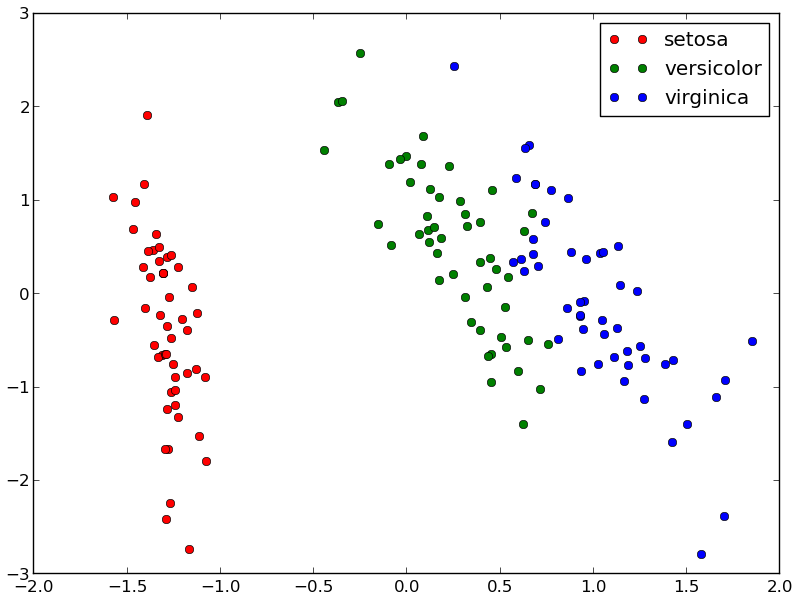
\includegraphics[width=\textwidth]{imgs/plot_iris.png} \\
       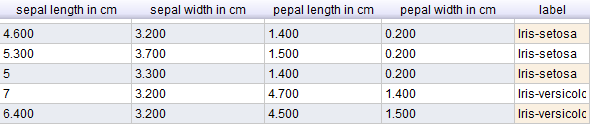
\includegraphics[width=\textwidth]{imgs/iris_dataset.png}
      \end{block}
     \end{column}
     
    \end{columns}

  \end{frame}


\subsection{Relevancia del problema}
  \begin{frame}
    \frametitle{Relevancia del problema}
    
    Todos los datos recolectados por una organización pueden ser útiles para
    mejorar las decisiones futuras de la organización. Para usar los enormes
    volúmenes de datos que se recolectan, es necesario encontrar patrones en
    ellos. La clasificación de datos se emplea en:
    
    \pause
    \begin{itemize}[<+->]
     \item Predicción de enfermedades
     \item Generación de perfiles de usuarios por empresas
     \item Toma de decisiones en una organización, minimizando riesgos empresariales
     \item Reducción de recursos dedicados al almacenamiento de datos por una empresa
    \end{itemize}
  \end{frame}
  

\section{Justificación del uso de IA}
  \begin{frame}
    \frametitle{Justificación del uso de IA}
      La mayoría de los cometidos que implican inteligencia requieren habilidad
      para extraer conocimiento de experiencias. En los problemas de clasificación
      resulta de gran importancia los llamados algoritmos de \textbf{machine learning},
      es decir, la extracción de información de manera automática estableciendo patrones
      que permitan efectuar una clasificación de datos. Por tanto, puesto que
      \textbf{clasificación} $\Longrightarrow$ \textbf{predicción}, estamos ante un claro problema de IA.
  \end{frame}

\section{Aplicaciones relevantes}
  \begin{frame}
   \frametitle{Aplicaciones relevantes}
   Según las características ausentes en los datos, la clasificación puede ser:
   \pause
   \begin{itemize}[<+->]
    \item \textbf{Binaria:} las instancias pertenecen a una de 2 clases (0-1, Verdadero-Falso). Ej.
      predicción de la diabetes a partir de datos médicos del paciente:
      \hlink{https://archive.ics.uci.edu/ml/datasets/Pima+Indians+Diabetes}{Pima Indians Diabetes}.
    \item \textbf{Multiclase:} se usa una característica con tantos valores como clases, de
      manera que se clasifican los datos en más de dos clases. Ej. reconocimiento de texto a mano alzada, en concreto un
    \hlink{https://www.kaggle.com/c/digit-recognizer}{Reconocedor de dígitos}
    \item \textbf{Multietiqueta:} cada instancia se puede asociar a más de una etiqueta ($\approx$ clase). Ej. clasificación de música según las emociones que transmite: \hlink{http://mlkd.csd.auth.gr/publication_details.asp?publicationID=269}{Emotions Dataset}
    
    % Nombrar multidimensional en la explicación
   \end{itemize}

   
  \end{frame}

  \subsection{Aplicación 1}
    \begin{frame}
      \frametitle{Diagnóstico de la diabetes}
      \begin{columns}[T]
       \begin{column}{.5\textwidth}
	 \justifying
	 Estudiar los atributos de personas que han padecido o no diabetes ayuda a
         la identificación de los factores de riesgo y la
         predicción del riesgo de un paciente concreto a desarrollarla según sus atributos.
         \\~\\
         Este es un problema de clasificación binaria. Los pacientes son divididos en aquellos
         de los que se predice que padecerán diabetes y aquellos que no.
         \\~\\
         Para resolver este caso se propone el uso de \textbf{árboles de decisión}. 
         
       \end{column}
       \begin{column}{.5\textwidth}
	  \begin{center}
	  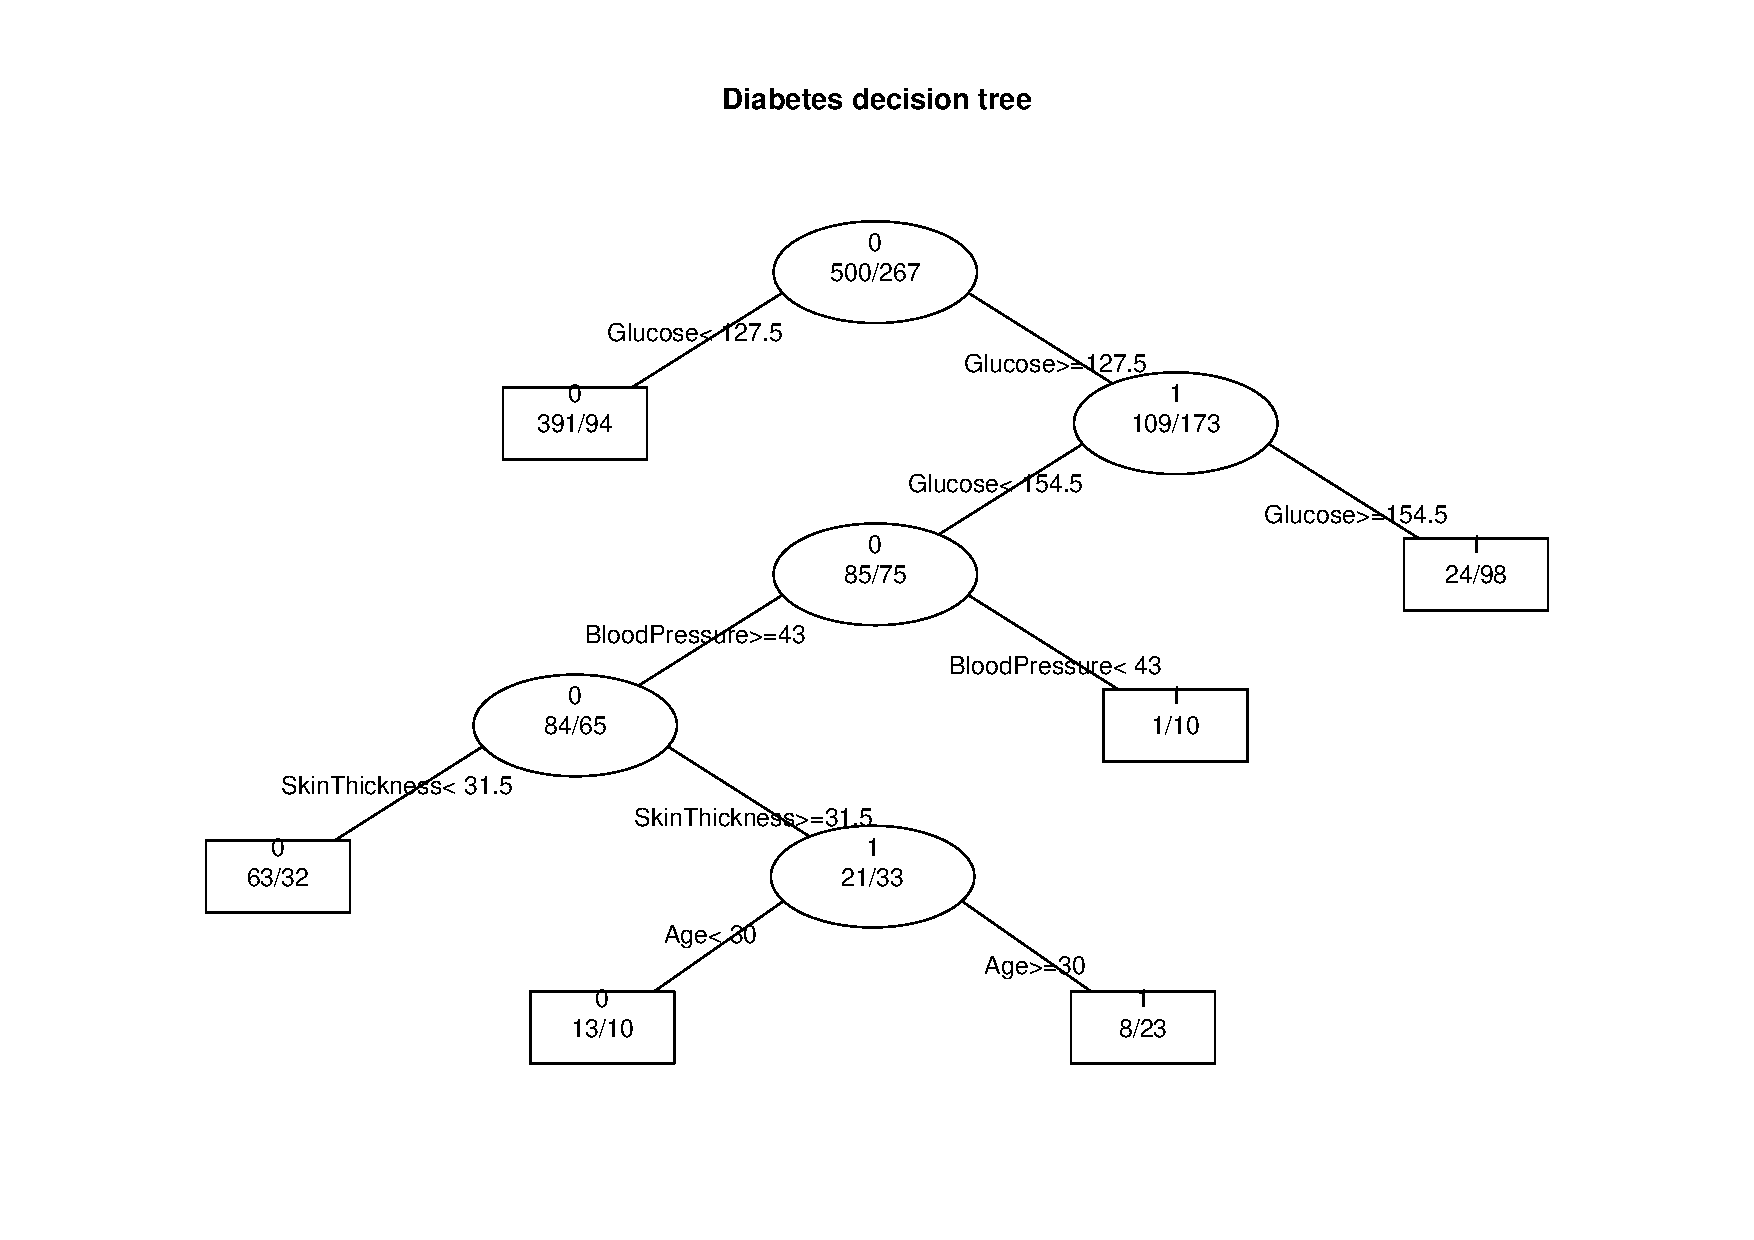
\includegraphics[width=\textwidth]{imgs/tree.pdf} % Generated in R
	  \\~\\
	  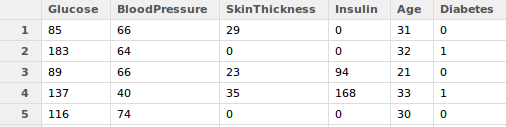
\includegraphics[width=\textwidth]{imgs/pima-indians-diabetes.png} % From http://cs-people.bu.edu/athitsos/nearest-neighbors/

	  \end{center}
       \end{column}
      \end{columns}
    \end{frame}
    
  \subsection{Aplicación 2}
    \begin{frame}
      \frametitle{Reconocedor de dígitos}
      \begin{columns}[T]
       \begin{column}{.5\textwidth}
	 \justifying
         El reconocimiento automático de dígitos y letras permite a los ordenadores
         leer entradas desde papeles manuscritos o fotografías.
         \\~\\
         Este es un problema de clasificación multiclase. Cada entrada deberá ser identificada
         como uno de los diez posibles dígitos.
         \\~\\
         Para resolver este caso se propone el \textbf{algoritmo KNN} (K-Nearest neighbors). 
         Ubicamos el dígito de entrada en un espacio métrico significativo y tomamos la clase mayoritaria 
         entre sus $k$ vecinos más cercanos. La inteligencia que exhibe el sistema vendrá
         determinada por la semántica del espacio métrico.
       \end{column}
       \begin{column}{.5\textwidth}
	  \begin{center}
	  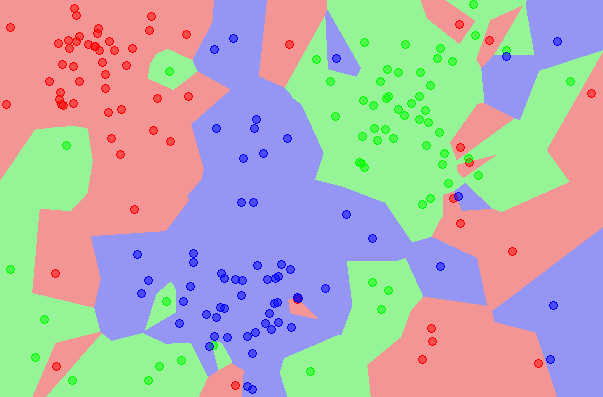
\includegraphics[width=.8\textwidth]{imgs/knn.png} % From http://en.wikipedia.org/wiki/File:Map1NN.png
	  \\ \centering \textit{KNN en dos dimensiones}
	  \\~\\
	  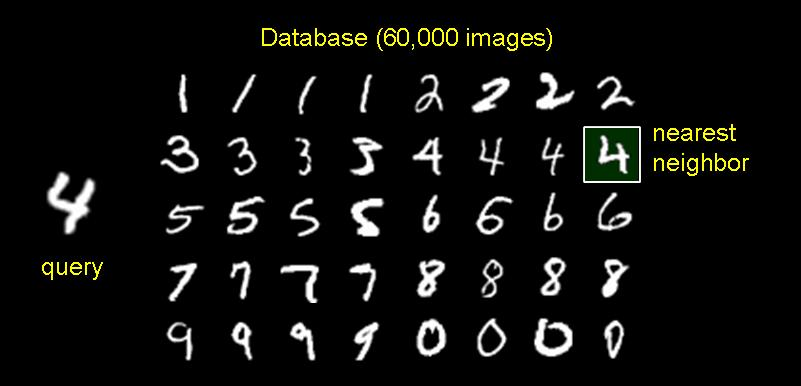
\includegraphics[width=.8\textwidth]{imgs/digit_database.jpg} % From http://cs-people.bu.edu/athitsos/nearest-neighbors/
	  \\ \centering \textit{Ejemplo de reconocimiento}
	  \end{center}
       \end{column}
      \end{columns}
    \end{frame}


\subsection{Aplicación 3}
  \begin{frame}
	\frametitle{Clasificación de música según emociones}
	\begin{columns}[T]
		\begin{column}{.5\textwidth}
			La detección de emociones en música se puede utilizar para la 
			\textbf{selección de música} a partir de alguna de las emociones que transmita.
			\\~\\
			Se modela como un problema de clasificación \textbf{multietiqueta}:
			cada canción puede inspirar más de una emoción
			\\~\\
			Las técnicas de preprocesamiento que se aplican aprenden de las
			\textbf{relaciones entre etiquetas} para alterar los datos y que
			un algoritmo de clasificación multietiqueta responda mejor.
			\\~\\
			\textbf{\textit{HOMER}} es un algoritmo que encuentra las etiquetas con mayor
			relación entre sí y las agrupa para construir problemas de clasificación
			más pequeños.
			
		\end{column}
		\begin{column}{.5\textwidth}
			\begin{center}
				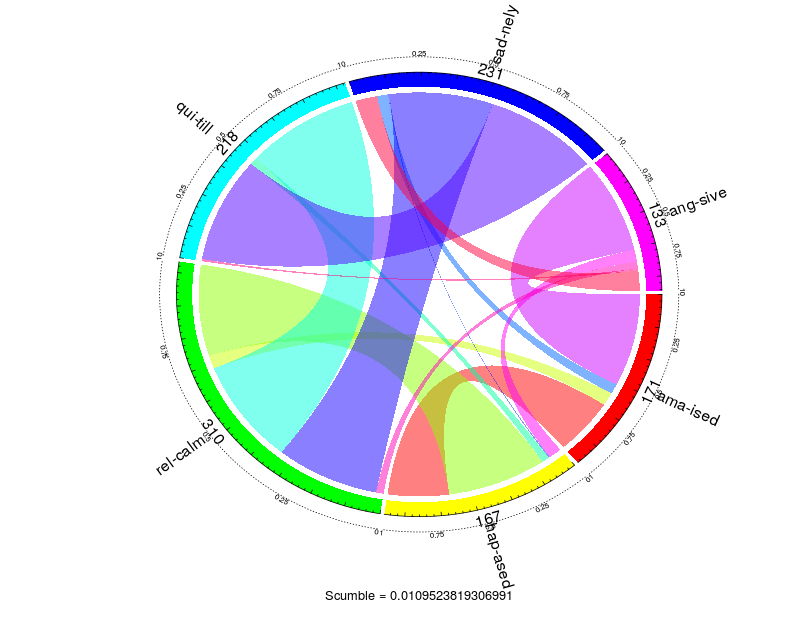
\includegraphics[width=.9\textwidth]{imgs/emotions-concurrence}
				\\ \centering \textit{Gráfico de concurrencia de etiquetas}
				\\~\\
				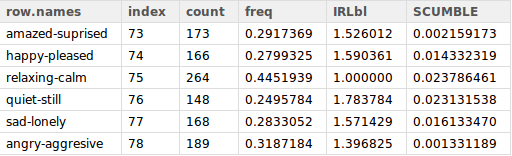
\includegraphics[width=.9\textwidth]{imgs/emotions-dataset}
				\\ \centering \textit{Etiquetas del dataset \texttt{emotions}}
			\end{center}
		\end{column}
	\end{columns}
  \end{frame}


%% Bibliografía
\section {Referencias}
\begin{frame}
\frametitle{Referencias}
\footnotesize{
  \begin{thebibliography}{99} % Beamer does not support BibTeX so references must be inserted manually as below
    \bibitem[Herrera, 2015]{h1} Francisco Herrera Triguero
      \newblock Inteligencia Artificial, Inteligencia Computacional y Big Data
      \newblock Capítulo A
      \newblock \emph{Universidad de Jaén (2015)}
      
      % Para la parte de clasificación. Está chulo eso de poder citarte a ti mismo en tu trabajo ;)
      % lol no hace falta esto, que va a quedar como que hemos reutilizado el 
      % trabajo en vez de hacer algo nuevo :O
     \bibitem[Charte]{c1} David Charte Luque
      \newblock Apuntes sobre Minería de Datos
      \newblock \hlink{https://github.com/dgiim/data-mining-classification}{data-mining-classification}
      \newblock \emph{Universidad de Granada (2014)}
  \end{thebibliography}
}
\end{frame}

\end{document} 